% Latex template: mahmoud.s.fahmy@students.kasralainy.edu.eg
% For more details: https://www.sharelatex.com/learn/Beamer

\documentclass[aspectratio=169]{beamer}					% Document class


\usepackage[english]{babel}				% Set language
\usepackage[utf8x]{inputenc}			% Set encoding
\usepackage{color}	
\usepackage{tikz}
\usepackage{amsmath}
\usepackage{amssymb}
\usepackage{bbm}

\usepackage{appendixnumberbeamer}


\newcommand{\Ell}{\mathcal{L}}
\newcommand{\mb}{\mathbf}
\newcommand{\ind}{\mathbbm{1}}
\newcommand{\E}{\mathbbm{E}}

\mode<presentation>						% Set options
{
  \usetheme{default}					% Set theme
  \usecolortheme{default} 				% Set colors
  \usefonttheme{default}  				% Set font theme
  \setbeamertemplate{caption}[numbered]	% Set caption to be numbered
  \beamertemplatenavigationsymbolsempty % Remove Nav Bar
  %\setbeamertemplate{footline}[frame number] % Add page number in footer
}

% \expandafter\def\expandafter\insertshorttitle\expandafter{%
%   \insertshorttitle\hfill%
%   \insertframenumber\,/\,\inserttotalframenumber}

% Uncomment this to have the outline at the beginning of each section highlighted.
%\AtBeginSection[]
%{
%  \begin{frame}{Outline}
%    \tableofcontents[currentsection]
%  \end{frame}
%}

\usepackage{graphicx}					% For including figures
\usepackage{booktabs}					% For table rules
\usepackage{hyperref}					% For cross-referencing

\title{Bayesian Optimization: A Review}	% Presentation title
\author{Fan Bu}			% Presentation author
\institute{}					% Author affiliation
\date{Lab meeting discussion, May 5 2023}	

\begin{document}

% Title page
% This page includes the informations defined earlier including title, author/s, affiliation/s and the date
\begin{frame}
  \titlepage
\end{frame}

% Outline (TOC)
% \begin{frame}{Outline}
%   \tableofcontents
% \end{frame}


%\section{Section One}

\begin{frame}{Roadmap}

\begin{itemize}
    \item The problem of global optimization with ``hard'' objective functions
    \item Logic and components of ``Bayesian Optimization''
    \item Technical details \& practical challenges
    \item Dicussion
\end{itemize}
    
\end{frame}

\begin{frame}{Problem: global optimization with limited evaluation budget}
	
	\begin{equation*}
		x^* = {\arg \max}_{x} f(x).
	\end{equation*}
\vspace{.5em}
	
	where $f(x)$ is assumed continuous, but
	\begin{itemize}
		\item ``black-box''
		\item expensive to evaluate
		\item doesn't admit gradients
		\item (dimension of $x \sim O(10)$ not huge \cite{frazier2018tutorial})
	\end{itemize}
	
	\pause 
	\vspace{.5em}
	
	
	\textbf{Goal}: find global optimizer $x$ with as few evaluations of $f$ as possible
	
\end{frame}

\begin{frame}{The logic of Bayesian Optimization}

Given data $\mathcal{D}_n = \{(x_n, y_n)\}$, evaluate $y_{n+1} = f(x_{n+1})$ at $x_{n+1}$ with highest gain:

	\vspace{.5em}

\begin{enumerate}
	\item ``approximate'' $f(x)$ with a statistical model
	\begin{itemize}
		\item usually a Gaussian process (GP)
	\end{itemize}
	\item find the next point $x_{n+1}$ to maximize an ``acquisition function'' 
	\begin{itemize}
		\item multiple choices balancing exploitation \& exploration
	\end{itemize}
\end{enumerate}
	
\end{frame}

\begin{frame}{Algorithm sketch}
	\begin{figure}
	\centering
	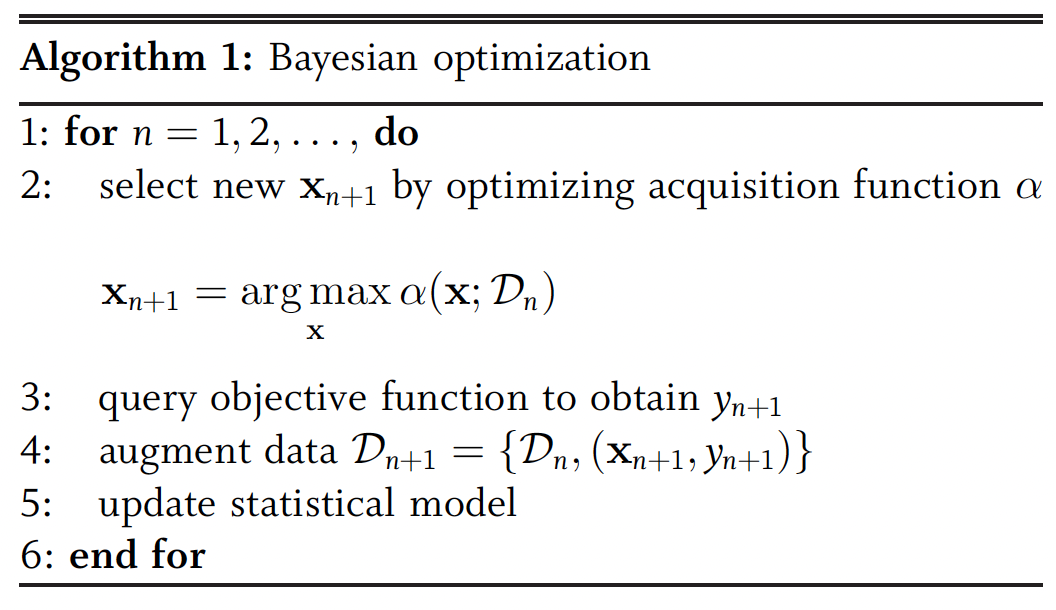
\includegraphics[width = 0.7\textwidth]{figures/Bo-alg1.png}
	\end{figure}
{
\footnotesize
Source: Shahriari et al., 2016 \cite{shahriari2015taking}. 
}

\end{frame}

\begin{frame}{Statistical model for $f(x)$}
	Common practice: GP model
	\begin{align*}
		y &\sim N(f(x), \sigma^2_{\text{noise}})\\
		f(x) &\sim \mathcal{GP}(\mu(x), k(x, x')).
	\end{align*}
	
	\begin{itemize}
		\item $\mu(x)$: mean function
		\item $k(x, x')$: kernel
		\pause
		\item \textbf{Closed-form predictive distribution} of $f(x_{\text{new}})$, conditioned on $\mathcal{D}_n$:
		\begin{equation*}
			f(x_{\text{new}}) \mid \mathcal{D}_n \sim N(\mu_n(x_{\text{new}}), \sigma^2_n(x_{\text{new}})).
		\end{equation*}
		\item (See pg.157, (29) \& (30) of \cite{shahriari2015taking})
	\end{itemize}

\end{frame}

\begin{frame}{Acquisition functions}
\textbf{In general}, choose next $x$ to maximize:
\begin{equation*}
	a \times \text{Exploitation term} + b \times \text{Explorartion term}.
\end{equation*}

Some common choices:
\begin{figure}
	\centering
	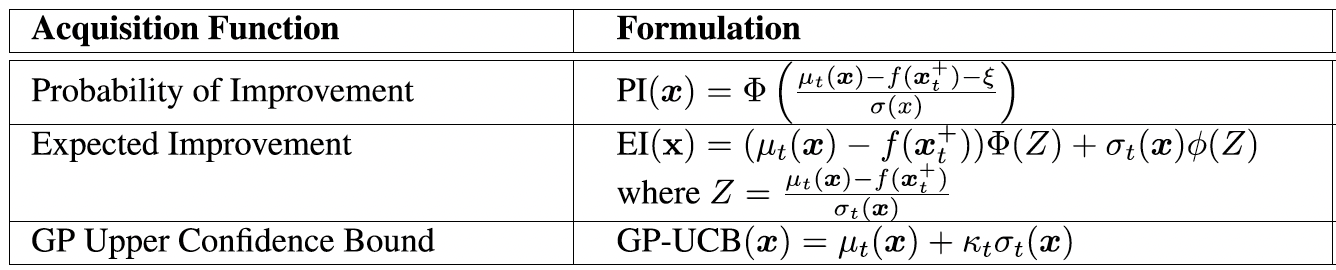
\includegraphics[width = 0.8\textwidth]{figures/acq-funcs.png}
\end{figure}

{
	\footnotesize
	Source: Greenhill et al., 2020 \cite{greenhill2020bayesian}. 
}
\end{frame}

\begin{frame}[plain]
	\begin{figure}
		\centering
		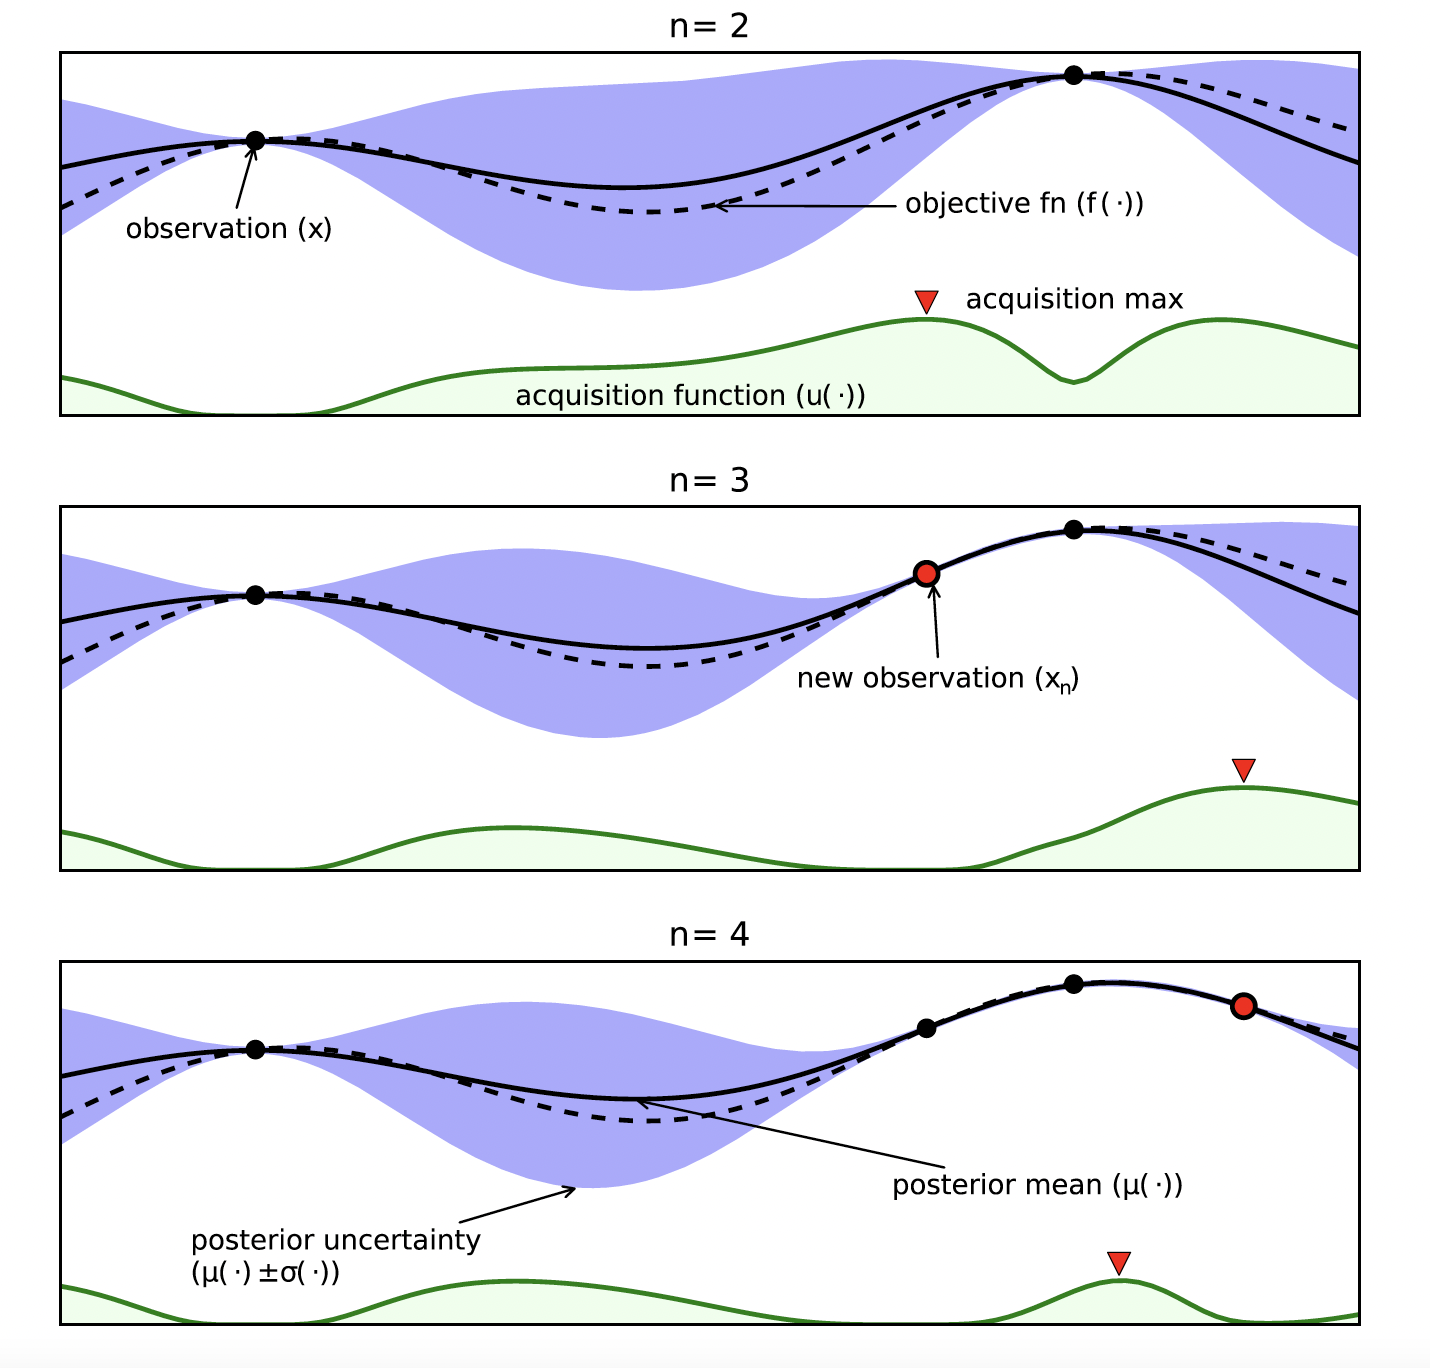
\includegraphics[width = 0.6\textwidth]{figures/BO-example.png}
		\caption{Example of BO in action. Source: \cite{shahriari2015taking}.}
	\end{figure}
	
	
\end{frame}

\begin{frame}{BO has a lot of applications}
	\begin{itemize}
		\item (Hyperparameter) Tuning of large/complex models, e.g.
		\begin{itemize}
			\item deep neural nets,  language models
		\end{itemize}
	\item Optimization/Simulation of complex dynamical systems, e.g., 
		\begin{itemize}
			\item systems in cosmology, meteorology, traffic flows
		\end{itemize}
	\item Online learning / reinforcement learning tasks, e.g., 
	\begin{itemize}
		\item A/B testing, recommender systems, etc.
		\item with connections to ``multi-armed bandits''
	\end{itemize}
	\item Experiment design in engineering (see \cite{greenhill2020bayesian} for a nice review)
	\end{itemize}
\end{frame}

\begin{frame}{The dirty truth: BO is hard}
	\begin{itemize}
		\item GPs are hard
		\begin{itemize}
			\item choice of kernel $k$
			\item hyperparameters of GP
			\item computational burden in inference (matrix inversion)
		\end{itemize}
		\item Acquisition function can be hard to optimize
		\begin{itemize}
			\item can be multi-modal and complex
			\item computational cost can be high
			\item (See Section V. B in \cite{shahriari2015taking} for review.)
		\end{itemize}
	\end{itemize}
\end{frame}

\begin{frame}{GP kernel choice}
	Usually stationary functions w.r.t. $r = \lVert x - x' \rVert_2$ for different levels of smoothness. See \cite{shahriari2015taking} pg. 157, (31-34) for examples. 
	
	\pause
	
	\begin{figure}
		\centering
		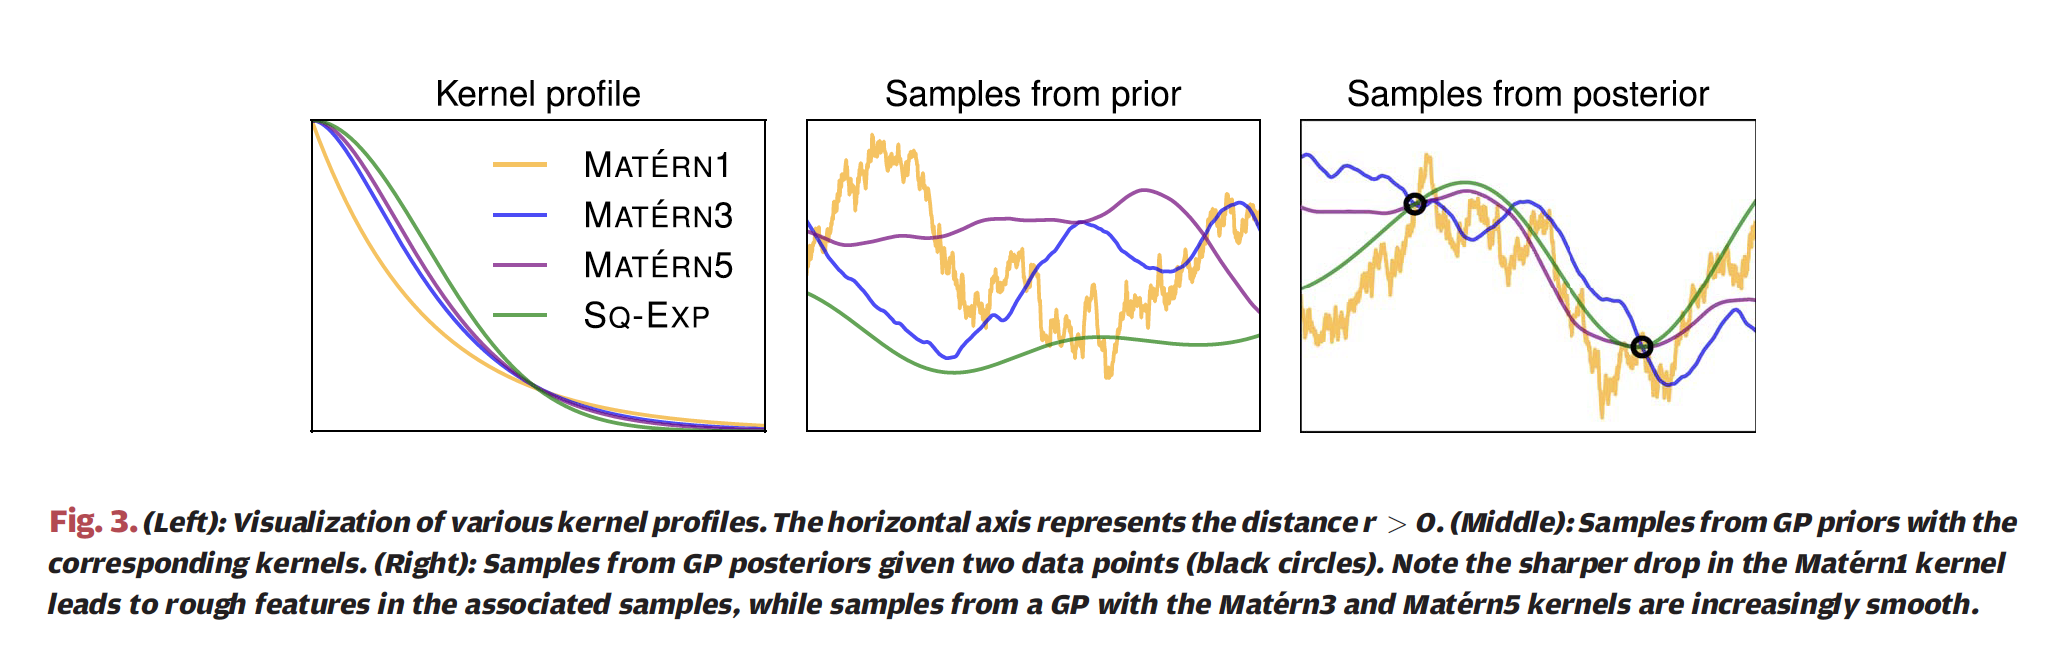
\includegraphics[width = 0.9\textwidth]{figures/kernel-function-examples.png}
	\end{figure}
	
	
\end{frame}

\begin{frame}{Handling hyperparameters}
	
	\textbf{Hyperparameters}: scale parameters in $k$, initial mean function $\mu_0$, noise variance $\sigma^2_{\text{noise}}$, etc.
	
	\vspace{1em}
	
	\begin{itemize}
		\item Optimal: marginalize over hyperparameters
		\begin{itemize}
			\item analytical solution if conjugate priors exist (and make sense)
			\item numerical solution through Monte Carlo simulation (or even MCMC)
		\end{itemize}
	\item Ad hoc: plug-in with estimates of hyperparameters
	\end{itemize}
	
\end{frame}

\begin{frame}{Computational burden}
	Each iteration of GP inference involves 
	\begin{equation*}
		\left[K + \sigma^2_{\text{noise}}I_n\right]^{-1},
	\end{equation*}
where $K \in \mathbb{R}^{n \times n}$ with $K_{i,j} = k(x_i, x_j)$. 	

\pause
\vspace{1em}

\begin{itemize}
	\item $O(n^3)$ if exact
	\item $O(n^2)$ with decomposition (e.g., Cholesky), \textbf{but} has to update every time
	\item $O(nm^2 + m^3)$ with approximation using $m$ pseudopoints (Section III. E. of \cite{shahriari2015taking}) 
	\item might further reduce if sparsity enforced (e.g., enforcing CAR-ish structure for conditional independence; similar to INLA \cite{rue2017bayesian})
\end{itemize}
\end{frame}

\begin{frame}{Parallelization}
	
	\begin{itemize}
		\item Pseudo-parallel: propose $J$ fantasies and get Monte Carlo estimate of $\alpha$; e.g., with EI \cite{snoek2012practical}. 
		\item Parallel: get a set of $J$ evaluation points simultaneously with various acquisition function tuning parameters; e.g, with GP-UCB \cite{hutter2012parallel, jones2001taxonomy}. 
		\end{itemize}
	
\end{frame}

\begin{frame}
	\begin{columns}
		\begin{column}{.6\textwidth}
				\begin{figure}
				\centering
				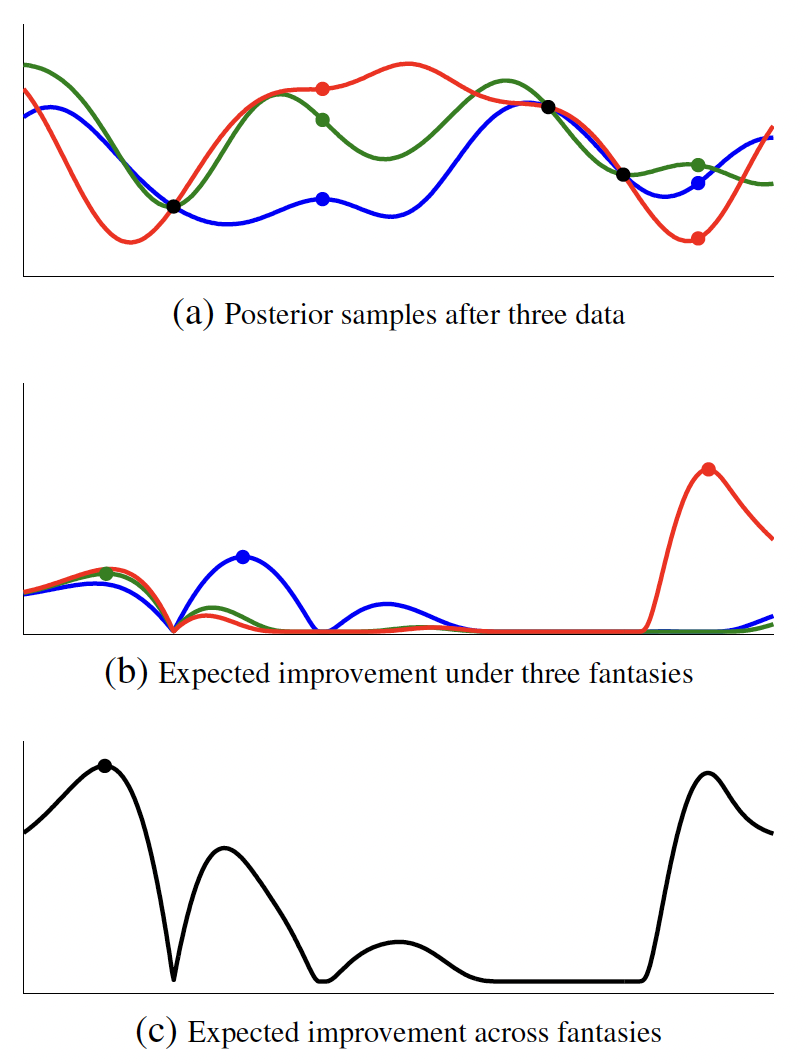
\includegraphics[width = 0.78\textwidth]{figures/fantasies-EI.png}
			\end{figure}
		\end{column}
	
		\begin{column}{.4\textwidth}
		Example: using 3 pending evaluations as ``fantasies'' to get ``expected'' acquisition function (EI in this example)
		\end{column}
	\end{columns}
\end{frame}


\begin{frame}{Discussion}
	\begin{itemize}
		\item High-dimensional case? 
		\begin{itemize}
			\item model order reduction techniques to reduce the ``effective dimensionality''?	
			\item e.g., cost-efficient online learning for splines...?
		\end{itemize}
		\pause
		\item Do we still care about uncertainty quantification? 
		\begin{itemize}
			\item can obtain/approximate marginal posterior of $x^* \mid \mathcal{D}_n$ 
		\end{itemize}
		\pause
		\item If pure exploration (no need for optimization)? 
		\begin{itemize}
			\item what happens if $\alpha := \sigma_n(x)$?
			\item next evaluation solely to reduce uncertainty
			\item (look more closely at $\sigma_n(x)$... )
			\item similar to mesh refinement in finite-element methods...? \cite{lo19983d,jones1997adaptive}
		\end{itemize}
		
	\end{itemize}
\end{frame}


\begin{frame}[allowframebreaks]{References}
 \bibliographystyle{amsalpha}
	\bibliography{references}

\end{frame}



\end{document}
